
\textbf{Problem 1:} stochastic processes
\begin{itemize}
\item[a)] [\textbf{2 points}] What is a stochastic process over a discrete, finite state space $\set{S} = \{ s_1, s_2, \ldots, s_m \}$ ? \\[4ex]
%%%%%
%%%%% enter your answer here
%%%%%
A set of random variables $\bigl\{ X_t \bigm| t \in \mathbb{N} \bigr\}$ where $X_t \in \set{S}$.





\vspace{8ex}
\item[b)] [\textbf{2 points}] What is a discrete time Markov chain (DTMC) ? \\[4ex]
%%%%%
%%%%% enter your answer here
%%%%%
A stochastic process such that for all $t \in \mathbb{N}$
\begin{equation*}
\cprob{X_t}{X_{t-1}, \ldots, X_0} = \cprob{X_t}{X_{t-1}} 
\end{equation*}
\end{itemize}
\newpage










\textbf{Problem 2:} Monte Carlo integration
\begin{itemize}
\item[a)] [\textbf{4 points}] Plot the gamma function
\begin{equation*}
\Gamma(z) = \int_0^\infty x^{z-1} \, e^{-x} \, dx
\end{equation*}
for $z \in \{ 1, 2, 3, 4, 5 \}$. \\[2ex]
%%%%%
%%%%% enter your answer here
%%%%%

\begin{center}
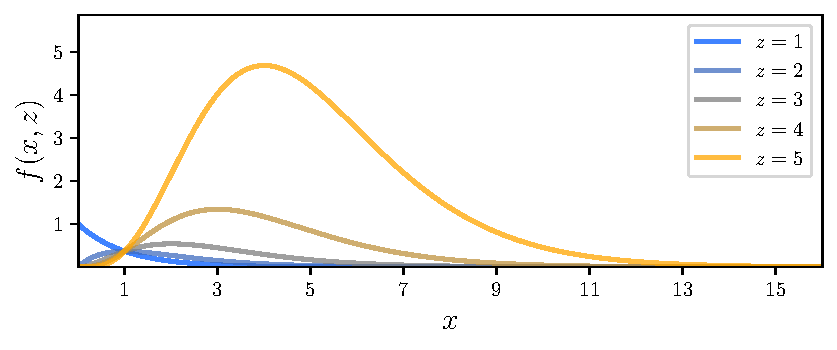
\includegraphics[width=0.9\textwidth]{gamma-integrant.pdf}
\end{center}





\vspace{8ex}
\item[b)] [\textbf{4 points}] Fill in the following table. \\[4ex]
%%%%%
%%%%% enter your answer here
%%%%%

\begin{center}
\begin{tabular}{c@{\hspace{3ex}}c@{\hspace{3ex}}c}
\toprule
$z$ & $(z-1)!$ & $\Gamma(z)$ \\
\midrule
$2$ & 1   & 1 \\
$3$ & 2   & 2 \\
$4$ & 6   & 6\\
$5$ & 24  & 24\\
$6$ & 120 & 120\\
\bottomrule
\end{tabular}
\end{center}





\newpage
\item[b)] [\textbf{4 points}] Show your python code for computing the entries of the above table. \\[4ex]
%%%%%
%%%%% enter your answer here
%%%%%
\begin{PythonCode}
import scipy as sp

for z in [2,3,4,5,6]:
	fact = sp.special.factorial(z-1)
	gamm = sp.special.gamma(z)
	print (fact, gamm)
\end{PythonCode}
\end{itemize}